\section{Wyniki i analiza badań}
To co wyszło i jak

\subsection{Rekonstrukcja - Gaussian Splatting}

\subsubsection{Wstęp}
Jak już wcześniej zostało wspomniane, algorytm posiada wiele hiperparametrów które mogą mieć różne optymalne wartości w zależności od sceny. Ogólnym więc zaleceniem jest uruchomienie algorytmu dla różnych wartości, a za pomoc mogą posłużyć poniższe wyniki naszych badań. 

Uwaga: do renderowania została użyta funkcjonalność biblioteki gsplat, więc wyniki mogą się różnić dla naszego własnego renderowania. 

\textbf{Przyjęte metryki}
\begin{enumerate}
    \item SSIM (ang. Structural Similarity Index Measure) - miara podobieństwa zdjęć, która bierze pod uwagę percepcyjne zjawiska np. związane z jasnością. Zakres wartości wynosi [-1, 1] wyższa wartość oznacza lepszą jakość. 
    \item PSNR (ang. Peak Signal-to-Noise Ratio) - stosunek maksymalnej mocy sygnału do mocy szumu zakłócającego ten sygnał, wyrażany w decybelach . Zakres wartości wynosi od 0 do $\infty$, wyższa wartość oznacza lepszą jakość. 
    \item LPIPS (ang. Learned Perceptual Image Patch Similarity) - metryka oparta na badaniach związanych z sieciami neuronowymi. Niższa wartość oznacza lepszą jakość. 
\end{enumerate}

\textbf{Eksperymenty dla sceny SKS}

Poniżej zostaną opisane wyniki różnych trenowań dla sceny SKS. 

\begin{table}[!h]
    \centering
    \begin{tabular}{|c|c|c|c|c|c|c|c|c|c|}
    \hline
    i & init\_opa & init\_scale & init\_type & scale\_reg & sh\_degree & sh\_interval & strategy & cap\_max & refine\_every \\
    \hline
    0 & 0.10 & 1.00 & sfm & 0.00 & 3 & 5000 & default & - & 100 \\
    \hline
    1 & 0.10 & 1.00 & sfm & 0.01 & 3 & 5000 & default & - & 100 \\
    \hline
    2 & 0.10 & 1.00 & sfm & 0.01 & 3 & 5000 & default & - & 500 \\
    \hline
    3 & 0.10 & 1.00 & sfm & 0.01 & 3 & 5000 & default & - & 1000 \\
    \hline
    4 & 0.50 & 0.10 & sfm & 0.01 & 3 & 5000 & default & - & 1000 \\
    \hline
    5 & 0.10 & 1.00 & sfm & 0.01 & 3 & 5000 & mcmc & 3000000 & 100 \\
    \hline
    6 & 0.10 & 1.00 & sfm & 0.01 & 3 & 5000 & mcmc & 3000000 & 500 \\
    \hline
    7 & 0.10 & 1.00 & sfm & 0.01 & 3 & 5000 & mcmc & 3000000 & 1000 \\
    \hline
    8 & 0.50 & 0.10 & sfm & 0.01 & 3 & 5000 & mcmc & 3000000 & 100 \\
    \hline
    9 & 0.50 & 0.10 & sfm & 0.01 & 1 & 5000 & mcmc & 3000000 & 100 \\
    \hline
    10 & 0.50 & 0.10 & sfm & 0.01 & 2 & 5000 & mcmc & 3000000 & 100 \\
    \hline
    11 & 0.50 & 0.10 & sfm & 0.01 & 2 & 5000 & default & - & 500 \\
    \hline
    12 & 0.50 & 0.10 & sfm & 0.01 & 1 & 5000 & default & - & 100 \\
    \hline
    \end{tabular}
    \caption{Konfiguracja trenowania dla sceny SKS}
    \label{table:tab_conf_sks}
\end{table}

W powyższej tabeli \ref{table:tab_conf_sks} uwzględnione są najważniejsze hiperparametry od których zależy jakość trenowania i końcowych wyników. 

\begin{table}[!h]
    \centering
    \begin{tabular}{|c|c|c|c|c|c|c|c|}
    \hline
    i & iteration & psnr & ssim & lpips & num\_GS & time (h) & size (MB) \\
    \hline
    0 & 19900 & 20.64 & 0.65 & 0.44 & 3,268,771 & 4.85 & 735.00 \\
    \hline
    1 & 11500 & 19.75 & 0.59 & 0.59 & 2,825,402 & 2.01 & 635.00 \\
    \hline
    2 & 46500 & 21.77 & 0.70 & 0.29 & 3,685,999 & 4.72 & 829.00 \\
    \hline
    3 & 71999 & 21.81 & 0.71 & 0.25 & 3,286,360 & 5.78 & 739.00 \\
    \hline
    4 & 63200 & 22.04 & 0.71 & 0.25 & 2,937,549 & 2.88 & 661.00 \\
    \hline
    5 & 56999 & 22.35 & 0.71 & 0.24 & 3,000,000 & 7.96 & 675.00 \\
    \hline
    6 & 41999 & 21.65 & 0.70 & 0.32 & 2,699,815 & 3.98 & 607.00 \\
    \hline
    7 & 89499 & 20.83 & 0.67 & 0.38 & 3,000,000 & 10.46 & 675.00 \\
    \hline
    8 & 31999 & 21.59 & 0.68 & 0.37 & 3,000,000 & 9.24 & 675.00 \\
    \hline
    9 & 44499 & 21.29 & 0.69 & 0.29 & 3,000,000 & 4.94 & 263.00 \\
    \hline
    10 & 56999 & 21.44 & 0.70 & 0.25 & 3,000,000 & 6.09 & 434.00 \\
    \hline
    11 & 51999 & 21.54 & 0.70 & 0.26 & 4,373,358 & 3.97 & 633.00 \\
    \hline
    12 & 14499 & 20.05 & 0.62 & 0.49 & 6,934,038 & 0.66 & 608.00 \\
    \hline
    \end{tabular}
    \caption{Wyniki eksperymentów dla sceny SKS}
    \label{table:tab_res_sks}
\end{table}

\pagebreak

\subsubsection{Zależność wyników od wartości hiperparametrów}

\textbf{Liczba Gaussianów}

\begin{figure}[!h]
    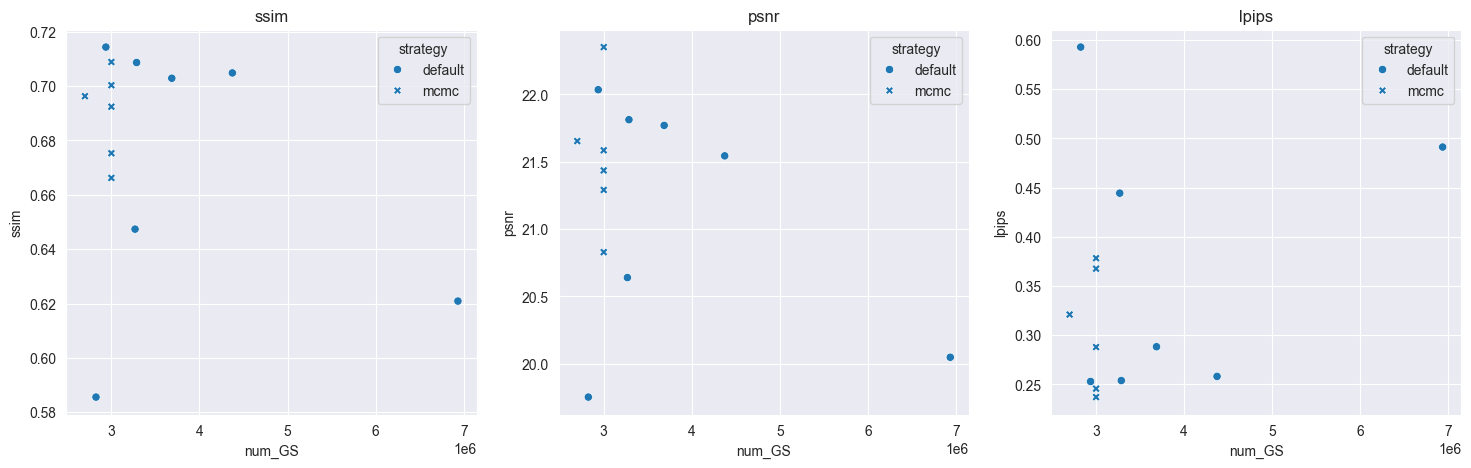
\includegraphics[width=\linewidth]{img/numGS_metrics.png}
    \caption{Zależność wartości metryk od liczby Gaussianów}
    \label{fig:metrics_1}
\end{figure}

Wyniki na powyższym wykresie mogą zaprzeczyć oczekiwaniu, że wraz z większą liczbą Gaussianów jakość sceny się polepsza. Zależy to również od strategii:
\begin{enumerate}
    \item default - strategia ta nie ma górnego ograniczenia na liczbę Gaussianów, co czasem może komplikować proces uczenia
    \item mcmc - strategia ta ma ograniczenie na liczbę Gaussianów, co może jednak sprawiać trudność dla użytkownika
\end{enumerate}

\textbf{Liczba iteracji}

\begin{figure}[!h]
    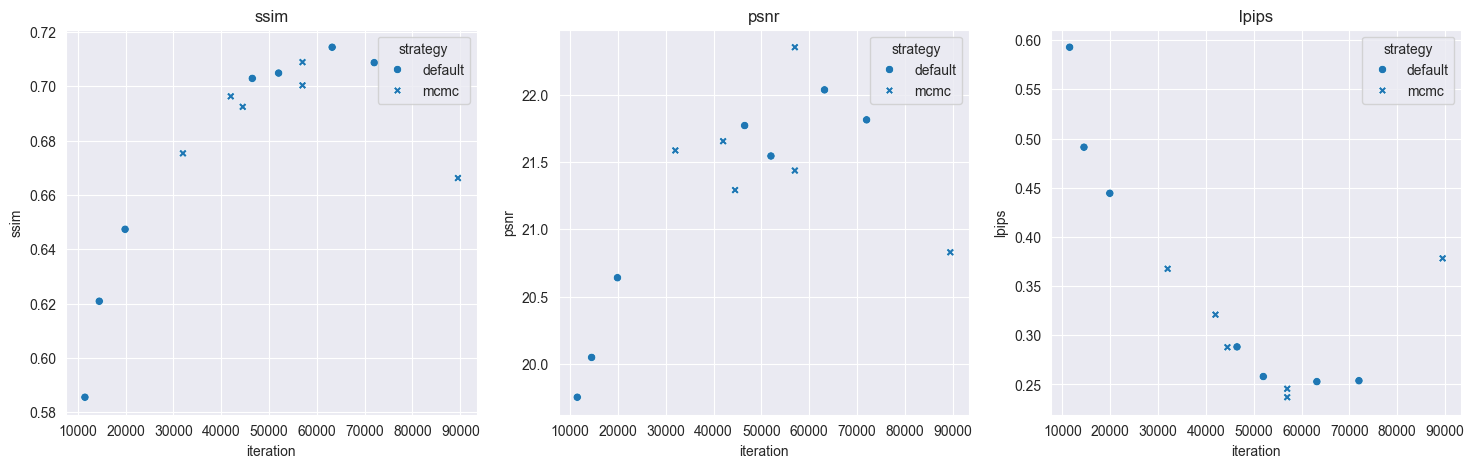
\includegraphics[width=\linewidth]{img/iterations_metrics.png}
    \caption{Zależność wartości metryk od liczby iteracji}
    \label{fig:metrics_2}
\end{figure}

W przypadku liczby iteracji widać trend polepszania się metryk wraz z większą ilością powtórzeń trenowania. 

\begin{figure}[!h]
    \centering
    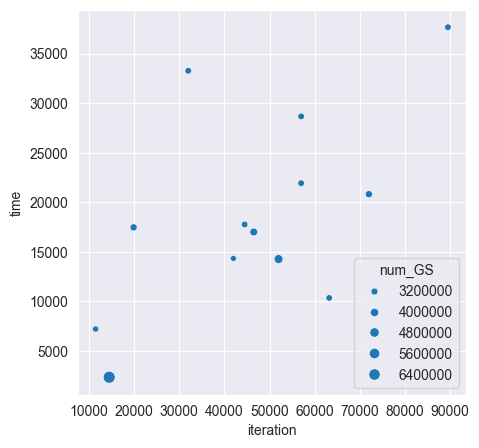
\includegraphics[width=0.6\linewidth]{img/training_time_iter.png}
    \caption{Czas trenowania w zależności od liczby iteracji}
    \label{fig:metrics_4}
\end{figure}

Istotne jest jednak podkreślenie tego, że dla tej samej liczby iteracji czas może być różny, co też wynika od np. przyjętej strategii czy też maszyny. Zwykle przyrost liczby Gaussianów w czasie był wykładniczy, co też wykładniczo wydłuża czas jednej iteracji. 

\textbf{Częstość adaptacji}

\begin{figure}[!h]
    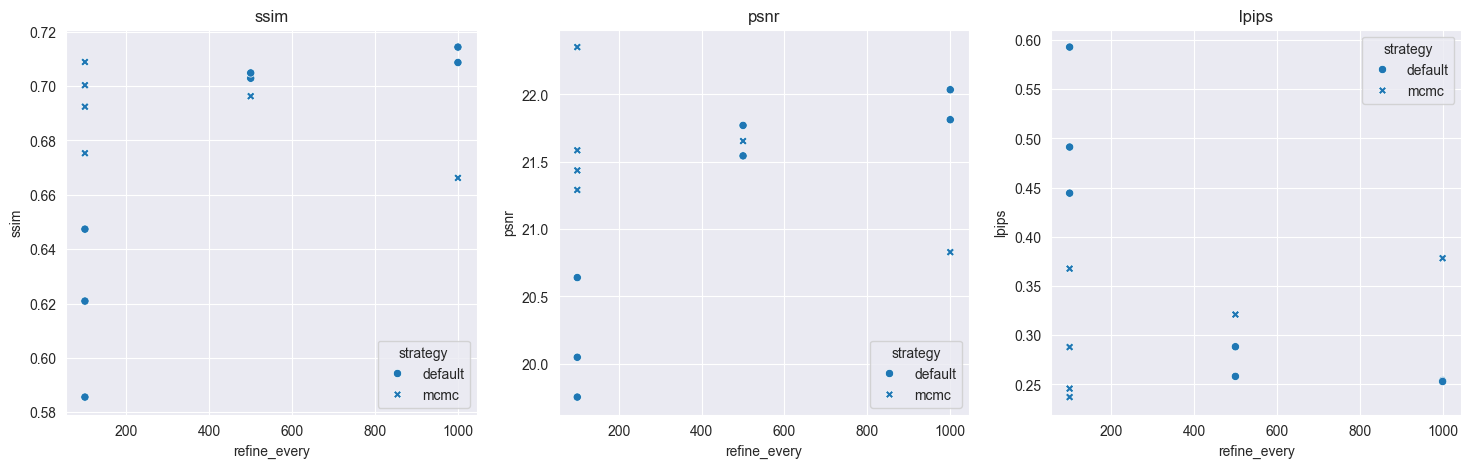
\includegraphics[width=\linewidth]{img/refine_every_metrics.png}
    \caption{Zależność wartości metryk od częstości adaptacji}
    \label{fig:metrics_3}
\end{figure}

Powyższe dwie zmienne - liczba Gaussianów oraz liczba iteracji - najbardziej są uzależnione od częstości adaptacji Gaussianów, ponieważ wtedy zachodzi dodawanie lub usuwanie Gaussianów. Testowane były wartości: 100, 500 i 1000. Ich zachowanie zależy od wybranej strategii: 
\begin{enumerate}
    \item default - jak już wspomniano strategia ta nie ma górnego ograniczenia na liczbę Gaussianów, co powoduje szybką ich proliferację bez pozytywnego wpływu na jakość sceny, więc zalecana jest wartość powyżej 500.
    \item mcmc - zalecana jest wartość poniżej 500, gdyż wtedy algorytm szybko osiągnie maksymalną liczbę Gaussianów i przez resztę iteracji będzie poprawiał ich parametry.  
\end{enumerate}

\textbf{Stopień zmiennych harmonicznych}
Prawie wszystkie eksperymenty zakładały wartość 3, co daje najlepszą jakość zdjęć, jednak za cenę zwiększonego zużycia pamięci i wydłużonego czasu trenowania. 

\pagebreak

\subsubsection{Porównanie zdjęć między eksperymentami}

\begin{figure}[!h]
    \centering
    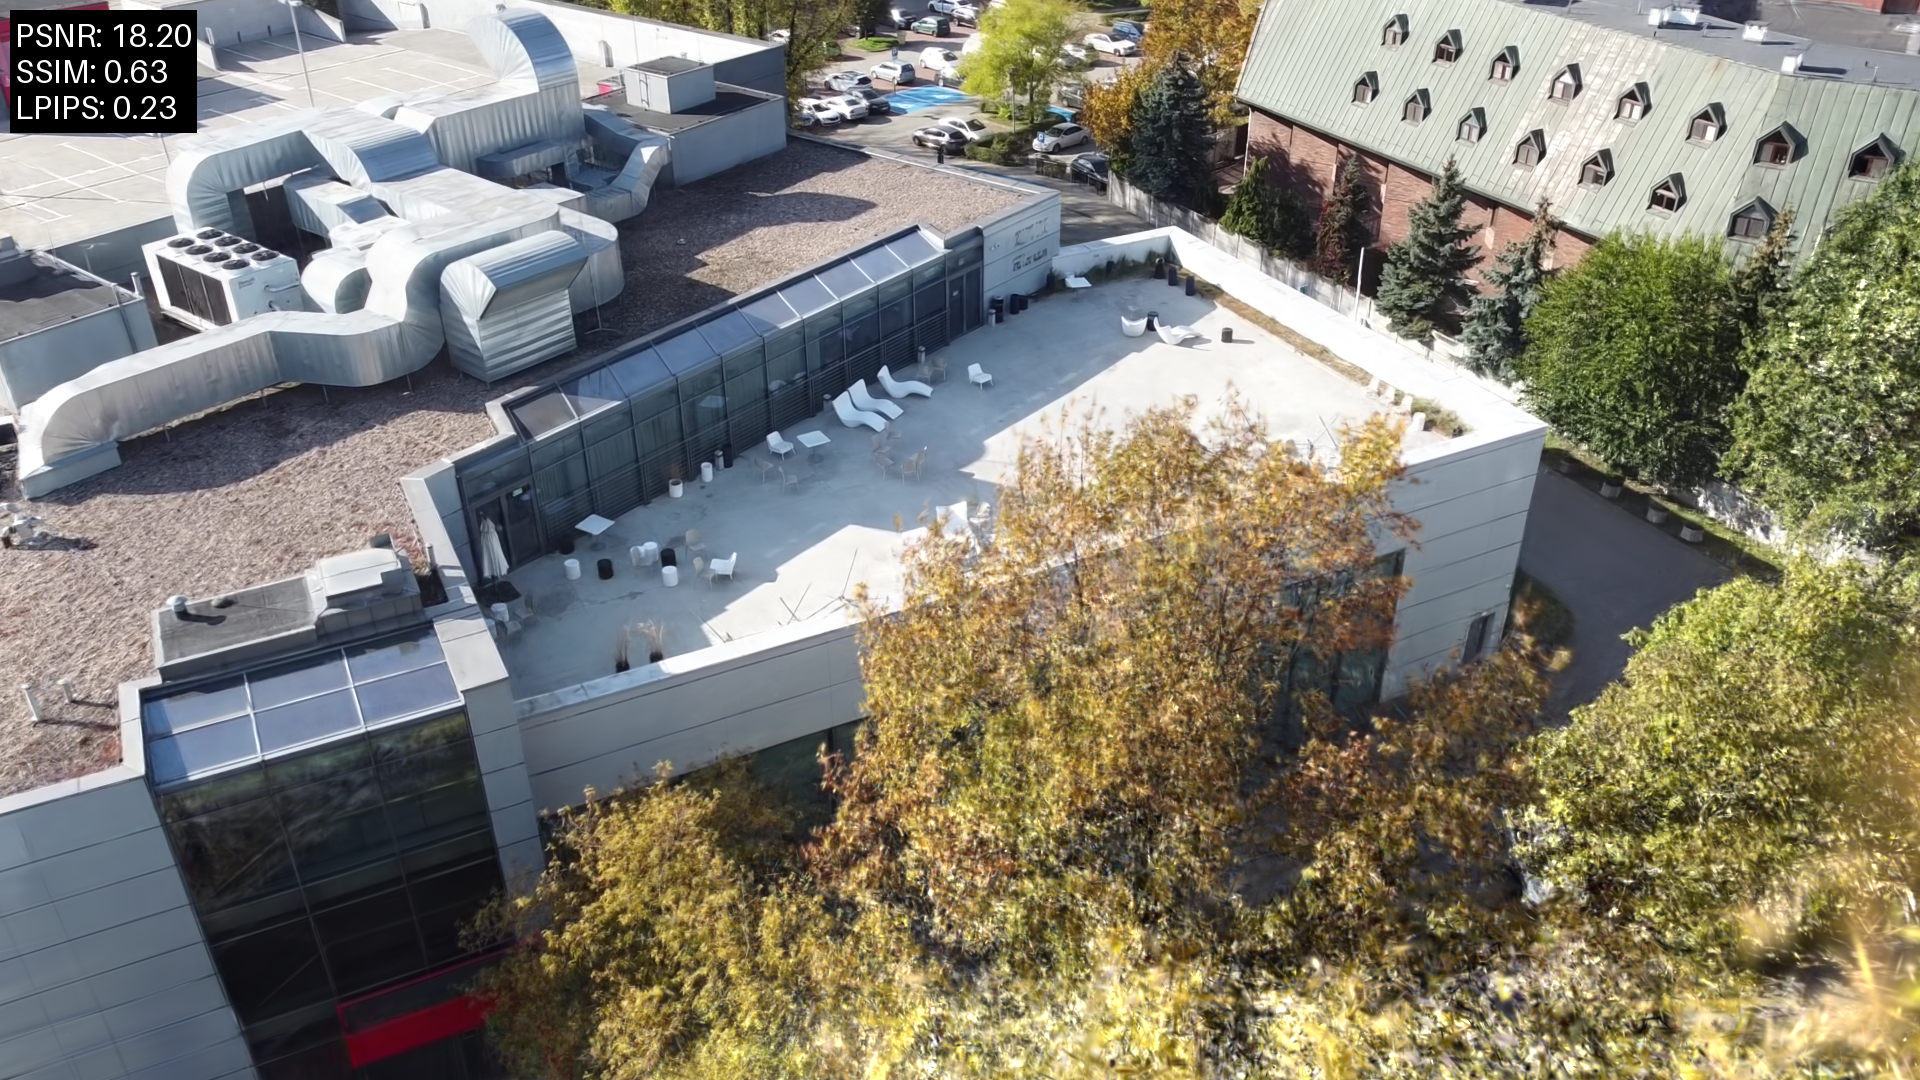
\includegraphics[width=0.8\linewidth]{img/res_imgs/eval_with_metrics_0010_5.png}
    \caption{Experyment i = 5 z najlepszymi metrykami}\label{fig:eval_1}
\end{figure}

\begin{figure}[!h]
    \centering
    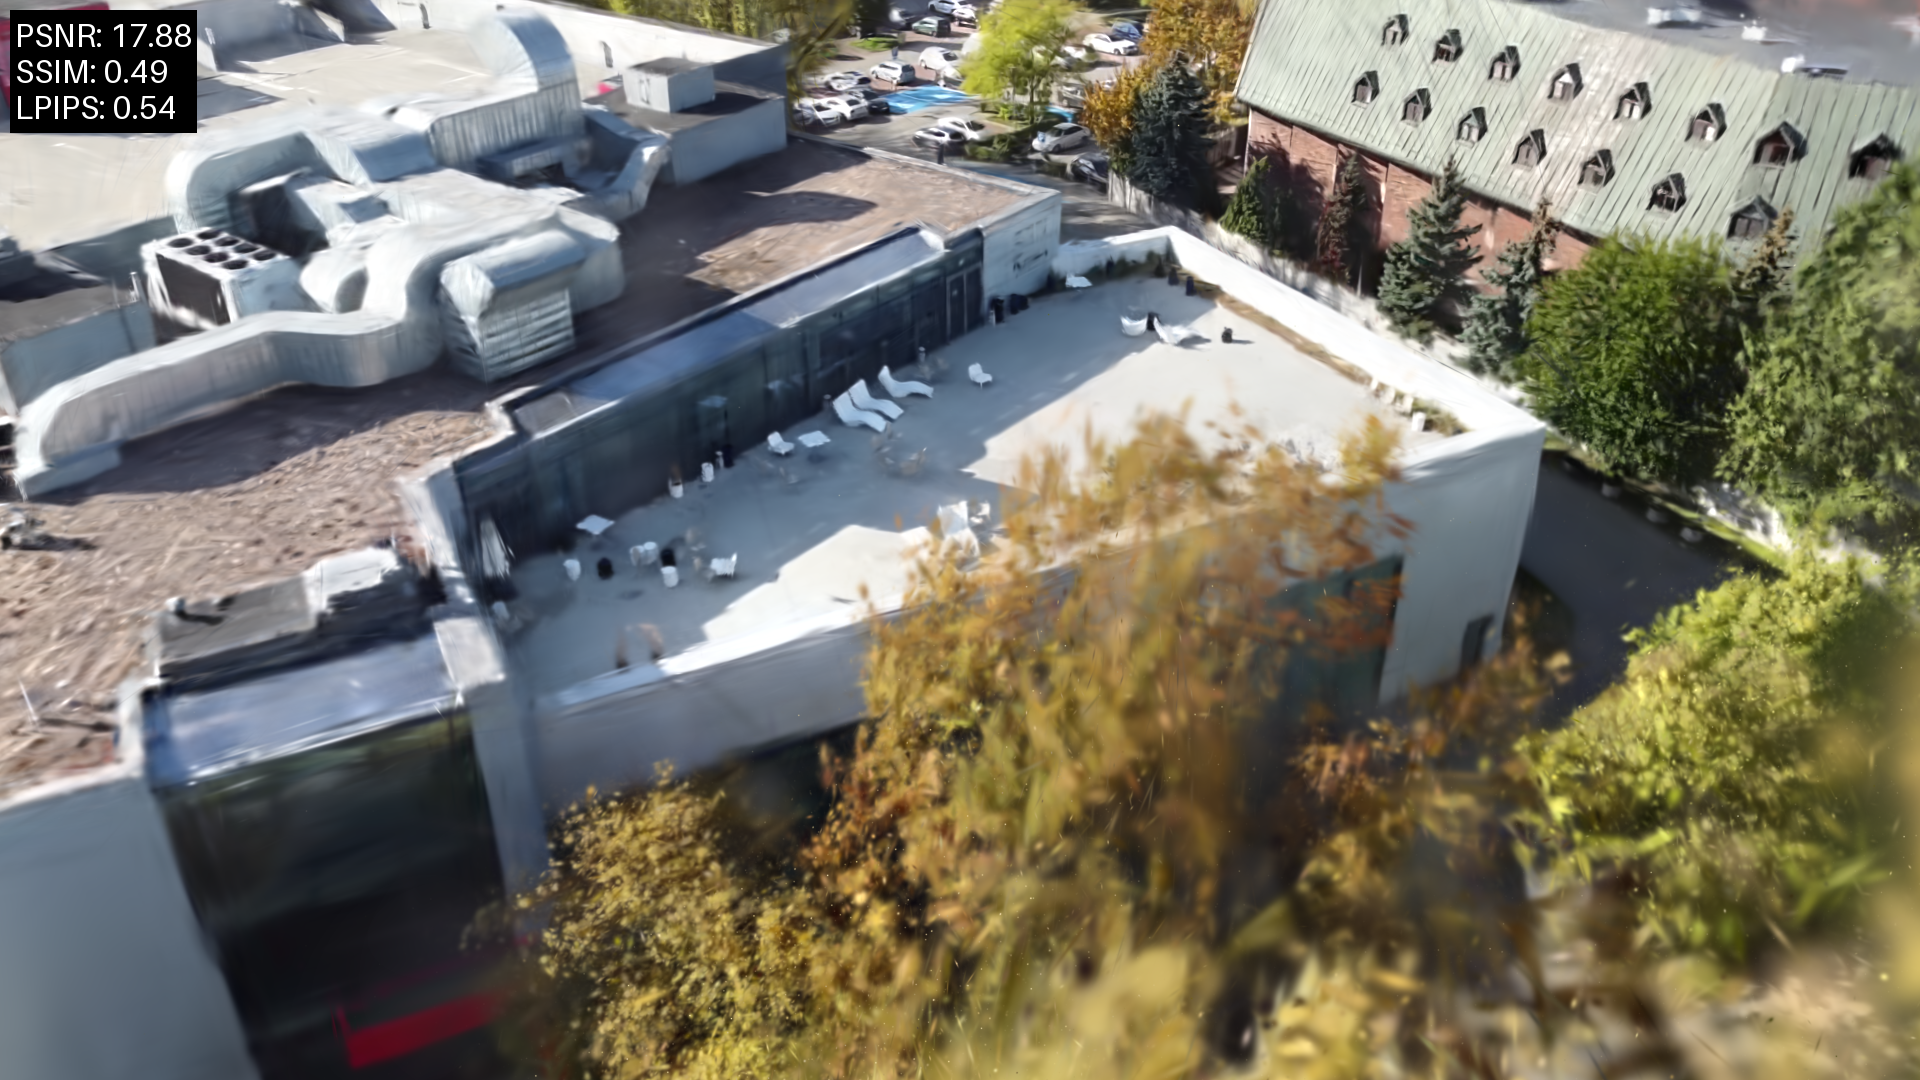
\includegraphics[width=0.8\linewidth]{img/res_imgs/eval_with_metrics_0010_1.png}
    \caption{Experyment i = 1 z najgorszymi metrykami}\label{fig:eval_5}
\end{figure}

Pierwsze zdjęcie z dobrą jakością pokazuje szczegóły jak np. krzesła, na drugim zdjęciu widoczne są artefakty spowodowane niewystarczającym dotrenowaniem gaussianów. 

\subsubsection{Podsumowanie}
Eksperymenty zostały przeprowadzone na jednej scenie ze względu na ograniczenia czasowe, jednak powyższe wnioski powinny się tyczyć również innych scen. \textit{gsplat} proponuje również inne parametry które mogą polepszyć jakość sceny, ale ze względu na ograniczenia nie zostały przetestowane. 